\setchapterpreamble[u]{\margintoc}
\chapter{Approach}
\labch{Approach}

%%%%%%%%%%%%%%%%%%%%%%%%%%%%%%%%%%%%%%%%%%%%%%%%%%%%%%%%%%%%%%%%%%%%%%%%%%%%%%%
%%%%%%%%%%%%%%%%%%% Motivation %%%%%%%%%%%%%%%%%%%%%%%%%%%%%%%%%%%%%%%%%%%%%%%%
%%%%%%%%%%%%%%%%%%%%%%%%%%%%%%%%%%%%%%%%%%%%%%%%%%%%%%%%%%%%%%%%%%%%%%%%%%%%%%%

\section{Motivation}
\labsec{motivation}

\todo{two stage approach be Ha and Schmidhuber 'world model'}

The basic approach of this work can be split into two steps:
\begin{enumerate}
    \item A differentiable renderer which can generate images of brush strokes from a parameter representation.
    \item An optimization procedure that iteratively approximates an image through brush strokes representations.
\end{enumerate}

The two step approach can be motivated by comparing the optimization procedure to the
actual process of painting an image.
An artist will most likely not pick single color particles to then place them on
the canvas.
Instead, the artist uses a brush or other utilities (see Pollock or others) to place
more paint with a single action.
\todo{image that shows different types of paint and tools etc.}
This of course limits the control over each individual drop of paint but maintains
enough control to still create very delicate details in paintings.
This trade-off varies for different brush sizes and for this reason an artist must
choose the brush size depending on the content.

An example would be the painting of a uniformly colored sky.
By using a large brush size the artist can cover a lot of canvas in relatively little
time as well as keep the color well distributed over the canvas because the brush
will spread color more or less evenly over its footprint.
On the other hand, if one were to draw a sky with the smallest brush available,
not only would it take forever to paint, it would also be hard to keep the paint
evenly distributed over multiple strokes.

Now, translating this onto the given problem of recreating/approximating an image
through brush strokes, it would mean to limit the process to only use what we would
describe as brush strokes. \todo{reformualte this}

An equivalent example would be the game of Tangram.

\begin{marginfigure}
    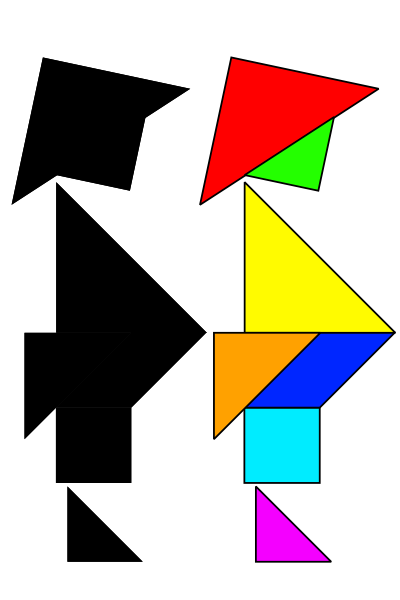
\includegraphics{tangram}
    \caption[]{An Example of Tangram.}
    \labfig{tangram}
\end{marginfigure}

Tangram is a Chinese puzzle game that has the objective of replicating a given silhouette
only with a set of 7 unique shapes.
The shapes may not overlay or be cut or anything.
Quite similarly, the objective for an optimizer is to replicate an image by only
using brush strokes.

\begin{marginfigure}
    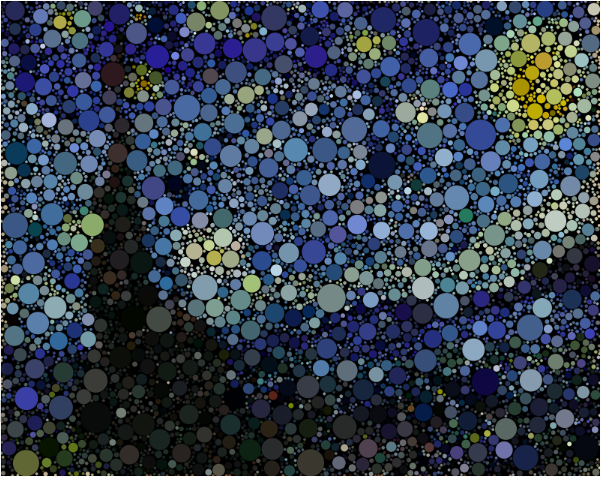
\includegraphics{genetic_starry_night}
    \caption[]{Starry Night approximated by a genetic algorithm using only circles. \url{https://effyfan.com/2018/03/02/w6-van-gogh-flowfield/}}
    \labfig{genetic}
\end{marginfigure}

This is a similar task to what genetic algorithms already can do and have done in
order to approximate images by other geometric shapes or even smaller photos (also 
known as the popular photo mosaic effect).
\paragraph{Genetic algorithms} follow a random sampling approach that 'evolves' like genomes do.
Basically starting with a random set of circles that are parameterized by their position,
radius and color; it then chooses the most successful samples and resamples again
in a region around these.
This process is repeated again and again, until a certain level of convergence is reached.

As well as this does work, it is very much computationally expensive as most samples
will not fit the image, thus searching for the tiny set fitting shapes requires
to evaluate all the bad shapes as well.
Since brush strokes have many more degrees of freedom and artworks usually consist
of upwards of a few thousand brush strokes this will not be applicable to this problem
until computational resources have become a few magnitudes more powerful.

\begin{figure}
    \includegraphics{photomosaic_starry_night}
    \caption[]{Photo mosaic of Starry Night using only images by the Hubble Space Telescope. \url{http://www.astro.uvic.ca/~alexhp/new/figures/starrynight_HST.001.jpg}}
    \labfig{photomosaic}
\end{figure}

This premise can be overcome, though, by using something that is known as as a differentiable
renderer.
\paragraph{Differentiable renderers} allow for the previously described task to be
feasible as random sampling is replaced by gradient descent.
A differentiable renderer is capable of creating shapes in the pixel domain by only
using differentiable operations.
Ordinary renderers do not have this property as they rely on faster operations that are
not differentiable as most renderers are not used in this context.
Also, creating a differentiable pipeline to render a circle from the tuple (position,
 radius, color) is a much harder task than calculation the shape of a circle beforehand
and then projecting the shape onto the pixels in an image and coloring them accordingly.
Nonetheless it is theoretically possible to create such a renderer.

Going back to the task of rendering brush strokes, it would be even harder to think
of a pipeline that uses only differentiable functions and is able to draw brush strokes
of a reasonable quality from a set of parameters.

This is where neural networks give an opportunity to avoid this problem.
Neural network are inherently differentiable and previous works have shown that
they are capable of high resolution and high quality conditional image generation.
One could easily think of a generator setup that takes as an input the parameters of
a brush stroke as well as some noise and then outputs an image of the according
brush stroke with possibly some variability in outline shape or other characteristics.

This principle was proposed by \cite{japanese neural renderer} as it facilitates
training of reinforcement learning based networks.

Inspired by this, the approach becomes more clear.
First, a differentiable renderer in form of a neural network is trained.
Then this renderer is used by an optimization procedure that uses gradient descent
to approximate an artwork as a input parameters batch of the renderer.

Both steps require some tricks to avoid pitfalls like computational limitation which
are outlined in the following two sections.

%%%%%%%%%%%%%%%%%%%%%%%%%%%%%%%%%%%%%%%%%%%%%%%%%%%%%%%%%%%%%%%%%%%%%%%%%%%%%%%
%%%%%%%%%%%%%%%%%%% Neural Renderer %%%%%%%%%%%%%%%%%%%%%%%%%%%%%%%%%%%%%%%%%%%
%%%%%%%%%%%%%%%%%%%%%%%%%%%%%%%%%%%%%%%%%%%%%%%%%%%%%%%%%%%%%%%%%%%%%%%%%%%%%%%

\section{Neural Renderer}
\labsec{NeuralRend}

The neural renderer is inspired by previous works (\todo{cite these works}) and 
is required to be differentiable and should be based on a rather simple architecture.
Especially since complicated architectures impose computational burdens and could
possibly distort the gradients for optimization.

\subsection{Data Set}
\labsubsec{dataset}

Unfortunately there is no data set available for this task which means that the data set
must be specifically created for this approach.

There are several sources for brush strokes that are evaluated in the following part.


\subsubsection{Brush Stroke Images}
\labsubsubsec{bsimages}

There are multiple sets of handrawn brush strokes available online.
Most notably there is a set of various well classified colors and brush styles created
by 'zolee' \todo{reference this} on the plattform \url{onlygfx.com}.
It cosists of approximately 1000 brush strokes that mostly follow rather straight
horizontal paths.
Brush strokes are mostly grouped by color and painting technique (oil, acrylic, watercolor...).
All images are in the PNG format and the area around the brush stroke was made 
transparent in a post-editing step.

This data set has the advantage that it consists of real world brush strokes that
were painted under presumably reproducible conditions.
On the other side, brush strokes are of mostly the same width throughout the data set
and also do not come with information which path the brush took or any other non-visual
information.
Also, the data is very sparse.
Many color shades are not represented which means that the generator would have to
'guess' them or simply would not be capable of rendering any brush strokes in this color.

It seems that this data set would be nice to replicate real world brush strokes
as images but limitations to the data make it unlikely that a generator could learn
a coherent representation from this.

\subsubsection{Painting Libraries}
\labsubsubsec{libmypaint}

The mentioned work of SPIRAL \todo{cite this} relies on opposite data to real world
images.
They used the painting library 'libmypaint' \cite{libmypaint} to generate brush strokes
from parameters in real time during training.

The obvious advantage of this and other painting libraries is the fact that one
can fully control the output through parameters.
This makes it much easier as the whole space of input parameters for the renderer
can be covered and avoids pitfalls like they were described in \ref{bsimages}.

Still, this data set falls short regarding the authenticity of rendered strokes.
Especially the inner area of the stroke shows a uniform color which is far from
what real brush strokes would look like.

This data set is better suited for our task than the given images are but will tend
to make all rendering look a bit 'cartoonish' or flat, which could in turn limit
convergence during the latter optimization process.

\subsubsection{Fluid Simulation}
\labsubsubsec{fluidpaint}

Fluid Paint \todo{cite website} is a project by \todo{name this guy} that uses simple
fluid dynamics to give artificial brush strokes a more plastic look.
It is implemented in JavaScript and OpenGL \todo{reference both}.

There is a C++ based version in the repository of SPIRAL which is also fitted with
python bindings by \todo{name that guy}.

Using these python bindings, it possible to generate brush strokes locally outside
of a web browser.

The quality and controllability of fluid paint falls right in between the two previously
mentioned datasets.
The generated brush strokes look distinctively better than those generated with 'libmypaint'
but still lack the quality of the real world images.
Concerning controllability, FluidPaint allows to control the path of the brush stroke
handle rather than the brush stroke itself.
This is a vast improvement over the images of 'zolee' but induces some offsets to
a given path as opposed to 'libmypaint'.

It seems that this is reasonable compromise between the previously mentioned data sets.
Although real time data generation in not possible with the library, it can be parallelized
to allow for the creation of large data sets in a reasonable time frame.

Even though this data set still has some weaknesses, it comes in as the probably best
choice for training a differentiable renderer because of the noted reasons.

\todo{add similar samples for all brush stroke methods.}

Other notable mentions are the painting programs \todo{these two weird software stuff things}
which allow for even more authentic brush strokes but lack a well documented interface
in order to generate a vast number of brush strokes.

\todo{talk about RGBA advantages}


\subsubsection{Brush Stroke Formalism}
\labsubsubsec{formalism}
With the means of data set production seized \todo{cut this joke}, what is left
is to formulate the parameters that define the brush strokes.
These parameters must quantify the following three properties of brush strokes:
\begin{itemize}
    \item color
    \item thickness
    \item path
\end{itemize}

The easiest of these three properties is quantifying the color.
Naturally, computer vision relies on the RGB format the defines color as a set of
three 8-Bit integer values between 0 and 255. 
As for path and thickness these two properties depend on the given coordinate system.
FluidPaint represents the canvas as a 2D plane in the $[0, 1]$ range, thus it makes
sense to follow the same representation.

Thickness thus becomes a value in $[0, 1]$  for each brush stroke, where 0 is and
infinitely small brush stroke and 1 is a brush stroke with the width of the canvas.
As both the edge cases do not make sense, the range is constrained to $[.03, .2]$
which includes only brush strokes that are visible and also do not cover the whole canvas.

Quantifying the path now is a little more tricky.
The fluid dynamics simulation that FluidPaint uses relies on internal time steps
at which the equations are evaluated and subsequently rendered.
At the same time each step allows only a linear motion of the brush handle between
positions $a$ and $b$.
This means that any curved paths must be split into linear/straight segments, that
should resemble a curved line.
As more steps mean longer simulation times and fewer steps mean edgy movement, a
value of 20 time steps per stroke is picked \todo{this is actually differernt as the steps depend on the lenght of the path. Look this up}.
This is equivalent to the number of steps that SPIRAL used in their implementation.

Another problem becomes how to express a curved path in numbers.
The easiest representation would be a sequence of points which make up the path of
interest.
This would give the highest versatility but at the same time introduce a noticeable
amount of parameters as each point consists of 2 coordinates rendering 40 values.
These values are also not independent but should follow are reasonable path as otherwise
the resulting brush stroke would look rather like a random walk than a believable
brush stroke.
Since works such as SPIRAL or Learning to Paint face a quite similar obstacle, their
solution should be applicable in this case as well.
Both works use so called 'Bezier curves' which parametrize curved paths by a limited
set of numbers.
\todo{image of bezier curve}

Bezier curves were invented in order to parametrize curved paths not through checkpoints
but analytical parametrizations for computer models.
They can be of different orders which allows them to follow more complicated paths
but in this case the simples form -- the first order -- is sufficient.
It defines a curve through its start and and point as well as a control point.
The curve is then defined as the path of a point over the time interval $[0, T]$.
First one connect the start and end points with the control point to get two lines
in return.
Along the lines on defines two points that move in a linear fashion along their lines
within the time interval $[0, T]$.
Then these two points are connected in the same way by a third line, which again
has a point moving along its direction over the span of $[0, T]$.
As the first two points that define the third line will move, the lines orientation
will change as well, thus translating the linear movement of the point into a complex
curved path.
The path that this point then takes in $[0, T]$ then defines the Bezier curve.
A first order Bezier curve will only bend into one direction or follow a straight path.
For higher orders the displayed process can be applied iteratively and allows for
more complex curves but as brush strokes usually follow a quite simple path and 
fewer parameters are preferred, Bezier curves of first order are chosen as parametrization.

Ultimately this gives 10 values that are sufficient to parametrize brush strokes
with certain constraints:
\begin{itemize}
    \item 3 two dimensional coordinates that define the Bezier curves (6 values).
    \item 1 thickness paramter.
    \item 3 values in RGB space.
\end{itemize}


\subsubsection{Data Constraints}
\labsubsubsec{constraints}

Given the parameters listed in section \ref{sssec:formalism}, the data still needs further
constraints to facilitate training of the generator even further.

Section \ref{sssec:fluidpaint} already hinted at the impracticality of online data generation.
A rough estimation by timing the rendering of 100.000 FluidPaint brush strokes reveals
that a dedicated CPU server is capable of generating 300 strokes per second when
using all of its resources.
\todo{experiment in appendix}
Keeping this in mind, a neural network with batch size 32 is limited to
$\approx 10$ terations per second which would mean a clear bottleneck.
Thus, it seems advisable to generate data beforehand with enough samples to cover
the data space sufficiently.
This will allow for much faster access to data, as individual data samples are relatively
small and can be stored in a binary data file such as HDF5.

Besides this constraint to the amount of data available, another set of constrains
will be introduced to reduce the data space to 'valid' brush strokes only.
'Valid' brush strokes will be defined as brush strokes which resemble real world
brush strokes to a certain degree.
This primarily concerns two relations within a brush stroke:
\begin{itemize}
    \item Its width-to-length ratio.
    \item Its curvature.
\end{itemize}

The width-to-length ratio will be restricted to brush strokes that are at least
two times as long as they are wide.
\begin{equation}
\norm{\vec{s} - \vec{e}} \overset{!}{\leq}  2 \times (\text{brush size}) \labeq{bs}
\end{equation}
Due to the simulation background of FluidPaint shorter brush strokes will show some
artifacts due to the bristles' length in the simulation which depends on the width
of the stroke.
Another reason for this, is the intended use case which will focus on van Gogh paintings.
As van Gogh did not practice pointillism most of his strokes have length to them,
which brings such a constraint in line with some characteristics of van Gogh's style.

The same argumentation can be done for the curvature:
Most brush strokes (especially those by van Gogh) have a certain 'flow' or 'smoothness'
to them, which can be described as by using strokes with large radii of their curvature
and without any corners in a strokes' path.
Thus data set will also be restricted to strokes which follow these descriptions.
In order to achieve this with random sampling in mind, a multivariate gaussian distribution
is placed between start point ($\vec{s}$) and end point ($\vec{e}$).
The two axes are rotated such that the short axis is in line with the vector
$\vec{a} = \vec{s} - \vec{e}$ while the other sits orthogonal.
Then both axes are scaled with $\norm{a}_2$ and also the handpicked values $\frac{1}{200}$
and $\frac{1}{25}$ for along $a$ and orthogonal to it, respectively.
Figure \ref{fig:datageneration} shows samples from this distribution for an exemplary
brush stroke.
\todo{draw figure in matplotlib or plotly or something}
This distribution is intended to follow that of brush strokes as they would appear
in the real world.
The majority of brush strokes will be straight or just slightly bent due to the maximum
of the PDF being at the center of $s$ and $e$.
Bent brush strokes will mostly be symmetric as the long axis of the multivariate gaussian
is orthogonal to $a$.
Still, there will be strokes that have their bent towards either end of the brush stroke
as well as some strokes with a high curvature.
The area of interest, though, will be densely populated as intended.
\begin{align}
    p(\vec{c}| \vec{s}, \vec{e}) & = \mathcal{N}(\mu, \Sigma) \labeq{checkpoint} \\
    \mu & = \frac{\vec{s} - \vec{e}}{2} + \vec{e} \\
    \Sigma & =
        \begin{pmatrix}
            \vec{a}_x & 0 \\
            0 & \vec{a}_y
        \end{pmatrix} \\
    \vec{a} & = \vec{s} - \vec{e}
\end{align}

The color of the brush strokes is not constrained as the color distribution of the
target data set is not known at this point. \todo{why not van gogh color distribution?}


%is this number of paramters enough, too much?

\subsubsection{Data Set Creation}
\labsubsubsec{creation}

The data set will be created with 100.000 samples that follow the constraints that
were presented in section \ref{sssec:constraints}.
As underlying distribution the uniform distribution is chosen as it allows a more
evenly coverage of the data space.

First, a set of start and end point as well as brush size is drawn and checked against
\eqref{eq:bs}.
If the constraint is not met, the set will be redrawn entirely.
In case the constraint is satisfied, a checkpoint is sampled according to \eqref{eq:checkpoint}.
If $\vec{c}$ lies outside the render window, the checkpoint will be resampled.
At last a color in form of an RGB value is sampled from a uniform distribution as well.

The resulting tuple of start, end and control point, brush size and RGB color is then
added to the data set.
Before rendering starts the values of $\vec{s}$, $\vec{e}$ and $\vec{c}$ are scaled
with the hand picked factor of $0.7$ to ensure the brush strokes are rendered completely
and not cut by the edge of the render window size.
At last the brush strokes are rendered according to the data set and added as well.
The render canvas size is 64x64 pixels.

As a last step, the data set is renormalized to the range $[-1, 1]$ for convenience
and to facilitate training as well.


\subsection{Architecture}
\labsubsec{arch}
The architecture of the brush stroke generator follows that of an inverse VGG network.
It is widely used and has shown in previous works that it should be capable of handling
this task.
\todo{check the details} The architecture consists of three dense layers at the beginning,
follow by an 2 times upsampling layer as well as three convolutional layers.
The same set of a 2 times upsampling layer and three convolutional layers is repeated
until the target size is reached.
After the last convolutional layer a tangens hyperbolicus function as applied, to
restrict the output to the $[-1, 1]$ range.
As part of the hyper-parameter search different tweaks to the architecture have been
tested:
\begin{itemize}
    \item An additional noise input at every layer with a size equal to that of the existing signal.
    \item Additional information about the position in the pixel grid in every layer, so called
        CoordConv \cite{coordconv}.
    \item Various combinations of activation and normalization functions.
\end{itemize}

\todo{network architectures as image}
The discriminator is designed after the same principles and resembles a VGG encoder
network
First three convolutional layers are applied, followed by a downsampling or pooling layer.
This is repeated until a target resolution of say 4x4 pixels is reached.
Then a set of three dense layers is applied to give one final prediction per sample.

\subsection{Training}
\labsubsec{train}
During training the L2 distance and the FID score were evaluated as metrics.
The FID score became necessary as the visual comparison of the generated samples
has proven difficult between different runs.
The L2 distance did not qualify as a sufficient metric for later training stages
as the stochastic nature of the brush strokes puts a threshold on how short the L2
distance can become.

To stabilize training further a two-time-step update rule was implemented.

\subsection{Results}
\labsubsec{results}

%%%%%%%%%%%%%%%%%%%%%%%%%%%%%%%%%%%%%%%%%%%%%%%%%%%%%%%%%%%%%%%%%%%%%%%%%%%%%%%
%%%%%%%%%%%%%%%%%%% Stroke Approximation %%%%%%%%%%%%%%%%%%%%%%%%%%%%%%%%%%%%%%
%%%%%%%%%%%%%%%%%%%%%%%%%%%%%%%%%%%%%%%%%%%%%%%%%%%%%%%%%%%%%%%%%%%%%%%%%%%%%%%

\section{Stroke Approximation}
\labsec{strokeapprox}

\subsection{Dataset}
\labsubsec{dataset}
First off, for this section the data set will be presented.
This is due to the data defining some demands for the networks later on.
The data set for the optimization task should also meet a few requirements.

In order to be able to focus on the brush strokes in an image the data set should
consist of relatively high resolution images.
This becomes necessary as most brush strokes should fit into a 64x64 window any larger
strokes could not be approximated with a single renderer and thus would falsely be constructed
of multiple brush strokes.

This requires more information per image than simply the resolution as the scale
of the image plays into this requirement as well.
Ideally each image should be accompanied by its size as this allows to rescale all 
images accordingly, given that one knows how large a typical brush stroke is.

At last the painting's technique must be oil on canvas or similar techniques as this
is what the renderer has been trained for.

All these requirements on the data can be met by using data directly from the Van
Gogh Museum in Amsterdam that is freely available online.
Each high resolution image is categorized by its technique as well as the period
in which it was painted accompanied by information on the measurements of the image.

\subsection{Weapon of Choice}
The next stage of training takes the now pre-trained neural renderer and combines
it with the task of approximating brush strokes in images.
In theory the neural renderer should allow to gather gradients in parameter space
even though meaningful losses are calculated in image space, as explained in section
\ref{sec:motivation}.
There, it was outlined already that the weapon of choice will be an optimization
procedure that relies on the capabilities of the neural renderer.

But this is not the only possible approach to dissecting images into sets op parameters.
As explained in \ref{sec:PR} there exist a variety of approaches for this kind of
task.
Some of these promise fast generation of parameters from images which makes the 
optimization approach in this work seem like a step back at first.
The following section is dedicated to justifying the chosen approach by comparing
state of the art implementations of existing approaches.

The targeted task is to approximate the representation of an image with roughly
1MP by the means of $\approx 10.000$ brush strokes (see section \ref{ssec:motivation}).

\subsubsection{Genetic Algorithms}
\labsubsubsec{genalg}
Genetic algorithms are possibly the simplest approaches.
As it was laid out in sections \ref{sec:motivation} and \ref{sec:genetic}, genetic
algorithms use random sampling and previous best results to approximate fitting
solutions to the rendering problem which was described in section \ref{sec:renderproblem}.

Current state of the art solutions are capable of finding a solution in $\approx 1h$,
when searching for an approximation of a 1MP image with simple geometric shapes
like circles or triangles.
This accounts for roughly $1 \times 10^{9}$ sampling steps
This time frame varies depending on target shape density, target accuracy, sampling
runs per shape and degrees of freedom (with the latter requiring more sampling runs).

Looking back at seciton \ref{sec:renderer} each brush strokes has 10 degrees of freedom
with some inter-dependencies between them.
Also it is known that the obtained neural renderer is capable of generating $\approx
300 \frac{\text{images}}{s}$.
This means that rendering the same amount of sampled images will take:
$$
\frac{10^{9} \text{samples}}{300 \frac{\text{images}}{s}} \approx 3.33 \times 10^{6} s
\approx 926 h \approx 38.6 d
$$
Which is an impossible amount of time to spend \textbf{per image}.

At this point the number of samples has not been corrected for by the higher number of
degrees of freedom of this problem.

Ultimately this means that genetic algorithms are not an option for this task.

\subsubsection{Brush Stroke Extraction}
\labsubsubsec{bse}
Next in the line of approaches are algorithm based approaches that use standard
computer vision techniques to extract brush strokes from an image and parametrize them.

Besides texton based image characterization \cite{textons} and pure filter based
approaches \cite{filters} there have been approaches to extract brush strokes or
some of their characteristics \cite{brushstrokecharacteristics} \cite{brushstrokeextraction}.

The latter would pose a valid option for the main goal of this thesis if it were to
characterize brush strokes reliably.
Unfortunately the best existing techniques fail to detect brush strokes equally 
over the whole image but only identify the most significant ones (see figure \ref{fig brushstrokeextracted}).
Other approaches are only able to extract only few characteristics like the orientation
of a brush stroke, which proves insufficient as well.
\todo{show some of the extracted brush strokes}

\subsubsection{Stroke Based Rendering}
\labsubsubsec{sbr}
A different field that also uses algorithm to approximate an image through brush strokes
and also wants to achieve some stylization along the way is Stroke Based Rendering
or Painterly Rendering.
While early works relied on interactive approaches, later publications then were able
to fully automate this process.
Judging from tests by the authors themselves such an approach would take between \todo{this number}
and \todo{this number} hours per image to fully render it this way.
As figures \ref{fig:sbr1} and \ref{fig:sbr2} show, these approaches obtain similar
results to genetic algorithms and tend to draw and image from a coarse scale to a finer scale
instead of locally coherent.

At last these approaches were not intended to be used to obtain brush strokes from
a painting but rather focus on stylizing images.
This renders such an approach unfit for the goal of this thesis as well.

\subsubsection{Drawing Networks}
\labsubsubsec{drawingnetworks}
Lastly, drawing networks are the newest iteration of approaches in this field.
Beginning with \todo{which one was first?} there have been approaches the make use
of feed-forward or recurrent neural networks combined with either supervised training
or deep reinforcement learning.
The best results by these approaches are shown in figure \ref{fig:drawingnets}.

Noticeably, all of these images have a maximum resolution of 256 pixels along the
longer edge.
There have not been any approaches yet, which are able to go significantly beyond
this limitation.
Especially, the high computational costs of training recurrent neural networks seems
to be an obstacle when shooting for higher resolutions.
As it will be outlined in more detail in \ref{ssec:dataset} such resolutions can not
be deemed sufficient when looking at individual brush strokes.

This, also rules out drawing networks.

\subsubsection{Combined Approach}
\labsubsubsec{combinedapproach}

Even though there have been plenty of previous approaches to the task of extracting
brush strokes from images or to similar task like rendering images through brush strokes;
none of these quite meet all the requirements that have been posed for this task.
Namely, high resolution input images, brush stroke focussed rendering and/or retrieval,
limited resources and realistic depiction of brush strokes.

Even though brush stroke extraction seems to be most fit for the main asset of
this thesis, stroke based rendering and drawing networks both bring features into
the mix, that seem capable of making the task at hand more feasible.
Drawing networks for once introduced differentiable renderers as a tool to facilitate
training.
Stroke based renderers achieve a parametrization implicitly by focussing on replicating
the entire image instead of extracting brush stroke by brush stroke.

This can be combined into a unified approach that uses the differentiable renderer
and the objective of recreating an entire image.
The resulting approach does not use re-sampling like genetic algorithms do, but
can rely on gradient descent to converge to a solution significantly faster.

The limited capabilities of such a renderer would also guarantee that any approximation
is composed of only valid brush strokes instead of single pixels it would be the
case with normal generative models.

All in all such an approach fits best to the goal of this thesis as it will generate
an approximation of a target image that ideally resembles the target as closely as
possible while being limited to the use of brush strokes.

\subsubsection{Pitfalls of Feed-Forward Approaches}
\labsubsubsec{ffapproaches}

In the course of this thesis there were experiments targeting a feed forward approach
before ultimately tending toward the optimization based approach that is presented.

The main reason for this change in direction can be pinpointed to two problems that
emerged.
The computational burden that of a feed-forward approach can be approximated when
looking at existing feed-forward approaches of drawing networks.
Without compromising resolution and this images quality significantly, training
a network can hardly be realized.
Still it was possible to show a basic implementation of this for very simple data
like the cMNIST data set. \todo{margin explain cmnist} \todo{add image that were drawn by ff network}

Another problem that occurred was the placement of brush strokes on the canvas.
As artists are not bound to the same pixel grid as images are, they can place brush
strokes freely on the canvas.
More so, they can pack brush strokes densely in one area while distributing them
broadly in another.

As most neural networks in computer vision are CNNs, they are not able to allow for
a similar behaviour as they will always follow a grid layout of various resolutions.

Repeated experiments with either displaceable grid cells or stacked signals have proven
too complicated to manage for a convolutional network architecture and also seemed
to scale badly when implemented in fully convolutional manner.

Thus an optimization based approximation was chosen as it offers good approximations
at high resolutions with manageable computational overhead.

\subsection{Optimization Based Approach}
\labsubsec{opt}
Since the previous section \ref{ssec:ffapproaches} already specified why an optimization
based approach has been chosen over a feed forward or recurrent approach, this section
is meant to explain a little more about the optimization procedure itself.

Fundamentally, it can be either compared to a stroke based rendering procedure or
it could be compared to the style transfer approach by Gatys \etal \cite{gatys}.

Starting with an initialization of brush strokes all brush strokes are optimized in
parallel to avoid any bias towards earlier brush strokes.
Each brush stroke is rendered as it is initialized using the differentiable renderer
introduced in section \ref{sec:NR}.

The outputs are then collected and build a so called render catalogue which holds
all rendering to the provided brush stroke parameters.

Together the parameter catalogue and the render catalogue are used to stitch the
individual renderings to a full image.
This requires to know the position of each brush stroke which is stored in the parameter
catalogue as well
 
\todo{introduce certainty}
\todo{introduce the principle of catalogues}
\todo{explain the limit due to computatioanl costs}

\subsubsection{Losses}
\labsubsubsec{losses}
\todo

\todo{sequential vs. parallel when explaining the optimization procedure}

\subsection{Image Composition}
\labsubsec{composition}

\todo{explain alpha blending}

\subsection{Results}
\labsubsec{results}

